\documentclass[a4paper, 12pt]{article}
\usepackage[left=2cm,right=2cm]{geometry}
\usepackage{times}
\usepackage[numbers]{natbib}
\usepackage[french]{babel}
\usepackage[utf8]{inputenc}
\usepackage[T1]{fontenc}
\usepackage{xcolor}
\usepackage{hyperref}

% listings support
\usepackage{listings}
\usepackage{verbatim}
\lstset{
  language=Java,
  extendedchars=true,
  inputencoding=utf8,
  basicstyle=\ttfamily,
  literate=
    {à}{{\`a}}1 {â}{{\^a}}1 {ç}{{\c{c}}}1 {é}{{\'e}}1 {è}{{\`e}}1
    {ê}{{\^e}}1 {ë}{{\"e}}1 {î}{{\^i}}1 {ï}{{\"i}}1 {ô}{{\^o}}1
    {û}{{\^u}}1 {ü}{{\"u}}1 {Ç}{{\c{C}}}1 {É}{{\'E}}1 {È}{{\`E}}1
    {Ê}{{\^E}}1 {Ë}{{\"E}}1 {Î}{{\^I}}1 {Ï}{{\"I}}1 {Ô}{{\^O}}1
    {Û}{{\^U}}1 {Ü}{{\"U}}1,
}

% to make nice graph figures
\usepackage{pgfplots}
\pgfplotsset{compat=1.18}
\usepackage{tikz}
\usetikzlibrary{shapes,arrows}
\usetikzlibrary{arrows.meta}

% formatting specifics
\setlength{\parindent}{0pt} % sets default to \noindent
% use \hspace{1em} for indentation
\usepackage{multicol}

% basic math package
\usepackage{amssymb}
\usepackage{amsmath}

% bibliography
\usepackage[numbib, nottoc]{tocbibind}
\bibliographystyle{plainnat}
\newcommand{\figref}[1]{(fig.\ref{#1}, p.\pageref{#1})}

% for figures and images
\usepackage{float}
\usepackage{graphicx}
\usepackage{graphbox}
\usepackage{adjustbox}
\usepackage{subfig} %use subcaption for better compatibility

\title{Projet de Traitement de Signal et Télécommunications \\
\Large Étude d’une chaîne de transmission sur porteuse pour une transmission
satellite fixe}
\author{Nicolas BAILLIET \and Paul LOUKA}
\date{30 mai 2024}

\begin{document}
\maketitle
\tableofcontents

% Vos rapports doivent comporter : un sommaire, une introduction présentant les
% objectifs du travail, une conclusion synthétisant les principaux résultats
% obtenus et une bibliographie comprenant les références éventuellement
% utilisées, notamment pour expliquer vos résultats. On peut y ajouter une table
% des illustrations.

\clearpage
\section{Introduction}

L'objectif de ce projet est d'étudier l'implémentation de chaînes de
transmission pour la diffusion de signaux numériques par satellite fixe. Nous
allons étudier et comparer plusieurs normes de transmission, notamment le DVB-S
et sa version plus récente DVB-S2, qui utilisent des mappings PSK, et une
alternative utilisant le mapping ASK.

\section{Implantation d'une transmission avec transposition de fréquence}

Commençons par étudier une transmission au format DVB-S, qui utilise un mapping
Quadrature Phase Shift Keying (QPSK) pour la modulation du signal. Ce mapping
est équivalent au 4-ASK à un déphasage de $\frac{\pi}{4}$ près. Par souci de
simplicité (permet une généralisation vers les M-PSK), nous utiliserons 4-PSK
pour la suite de l'étude, les résultats obtenus étant équivalents. \medbreak

La chaîne de transmission suit le schéma suivant :

\begin{figure}[H]
    \centering
    \begin{tikzpicture}
        \tikzstyle{block} = [rectangle, draw, text width=6.5em, text centered, rounded corners, minimum height=4em]
        \tikzstyle{line} = [draw, -{Latex[length=2mm]}]

        \node [block] (mapping) {Mapping};
        \node [block, right of=mapping, node distance=4cm] (filtreemission) {Filtre d'émission \\ $h_e$};
        \node [block, right of=filtreemission, node distance=4cm] (transposition) {Transposition de fréquence $f_p$};
        \node [block, right of=transposition, node distance=4cm] (transmission) {Transmission};
        \node [block, below of=transmission, node distance=3cm] (reception) {Retour en bande de base};
        \node [block, left of=reception, node distance=4cm] (filtrereception) {Filtre de réception $h_r$ adapté};
        \node [block, left of=filtrereception, node distance=4cm] (echantillonnage) {Échantillonnage optimal};
        \node [block, left of=echantillonnage, node distance=4cm] (demapping) {Démapping};

        \path [line] (-2, 0) -- node[midway, below, yshift=-1cm] {Bits de débit $R_b$} (mapping);
        \path [line] (mapping) -- node[midway, below, yshift=-1cm] {Symboles} (filtreemission);
        \path [line] (filtreemission) -- node[midway, below, yshift=-1cm] {Signal complexe} (transposition);
        \path [line] (transposition) -- node[midway, below, yshift=-1cm] {Signal réel} (transmission);
        \path [line] (transmission) -- node[midway, right] {Signal réel} (reception);
        \path [line] (reception) -- node[midway, below, yshift=-1cm] {Signal complexe} (filtrereception);
        \path [line] (filtrereception) -- node[midway, below, yshift=-1cm] {Signal complexe} (echantillonnage);
        \path [line] (echantillonnage) -- node[midway, below, yshift=-1cm] {Symboles} (demapping);
        \path [line] (demapping) -- node[midway, below, yshift=-1cm] {Bits} (-2, -3);
    \end{tikzpicture}
    \caption{Chaîne de transmission}
\end{figure}

Le filtre d'émission $h_e$ est en racine de cosinus surélevé, de roll-off
$\alpha = 0.35$. Le filtre de réception $h_r$ est adapté à $h_e$. Tout au long
de l'étude, il vérifie $h_r = h_e$ car nous ne considérons pas de filtre de
canal. Dans cette partie nous avons $f_p = 2kHz$, $R_b = 3kbps$ et une fréquence
d'échantillonnage $F_e = 24kHz$. \medbreak

Avec le mapping 4-PSK, nous obtenons des symboles complexes de la forme $d_k =
a_k + jb_k$ avec $a_k \in \{-1, 1\}, \, b_k \in \{-1, 1\}$. Nous avons donc un
signal qui se décompose en deux signaux réels en quadrature de phase.

\clearpage
\vspace*{-2cm}
\begin{figure}[H]
    \centering
    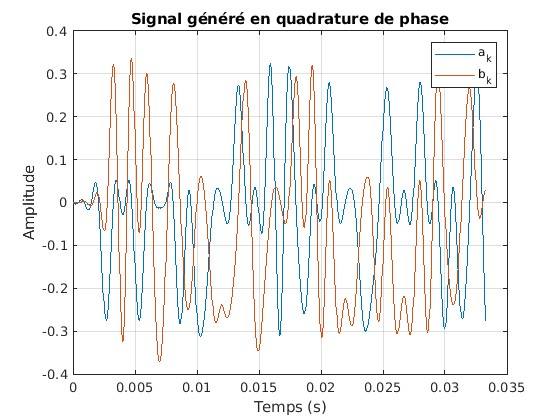
\includegraphics[width=0.7\textwidth]{graphics/1-1.jpg}
    \caption{Signaux réels issus du mapping QPSK}
    \label{fig:sig_quad}
\end{figure}

Une fois le signal transposé sur la fréquence $f_p$ et converti en signal réel,
nous obtenons le signal émis suivant:

\begin{figure}[H]
    \centering
    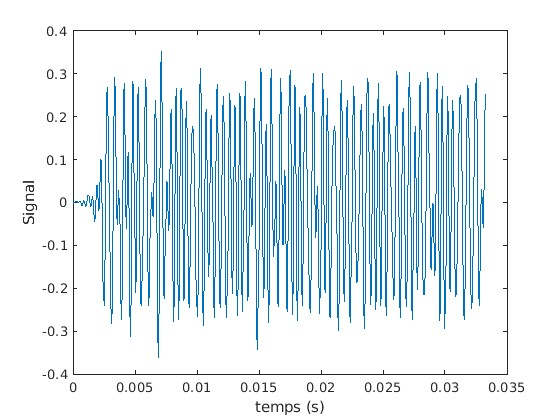
\includegraphics[width=0.7\textwidth]{graphics/1-2.jpg}
    \caption{Signal transmis sur fréquence porteuse}
    \label{fig:sig_porteuse}
\end{figure}

On peut visualiser la densité spectrale de puissance du signal transmis sur la
fréquence porteuse:

\begin{figure}[H]
    \centering
    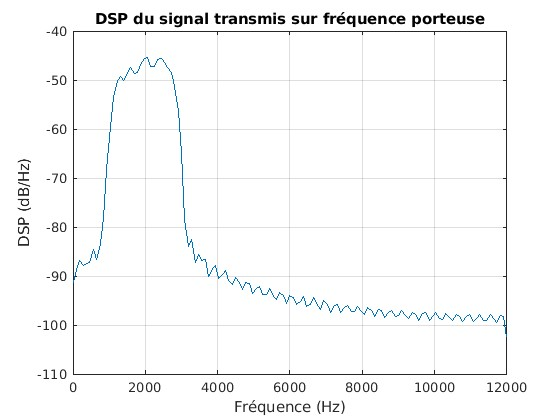
\includegraphics[width=0.7\textwidth]{graphics/1-3.jpg}
    \caption{DSP du signal transmis sur fréquence porteuse}
    \label{fig:sig_porteuse_dsp}
\end{figure}

On observe bel et bien un signal centré autour de $f_p = 2kHz$. La forme de la
DSP correspond à la transformée de Fourier d'une racine de cosinus surélevé, i.e.
notre filtre d'émission $h_e$. \medbreak

Le signal transmis dans le canal subit un bruit additif blanc gaussien, de
puissance \[ \sigma^2 = \frac{P_x N_s}{2 \log_2(M) \operatorname{SNRB}} \] avec
$P_x$ la puissance du signal, $N_s$ le nombre d'échantillons par symbole, $M$
l'ordre de modulation et $\operatorname{SNRB}$ le rapport signal sur bruit par
bit à l'entrée du récepteur. \medbreak

Le signal reçu est ensuite transposé en bande de base, puis filtré par le filtre
de réception $h_r$ adapté. Pour finir, évaluons le Taux d'Erreur Binaire (TEB)
en fonction du $\operatorname{SNRB}$. \medbreak

\begin{figure}[H]
    \centering
    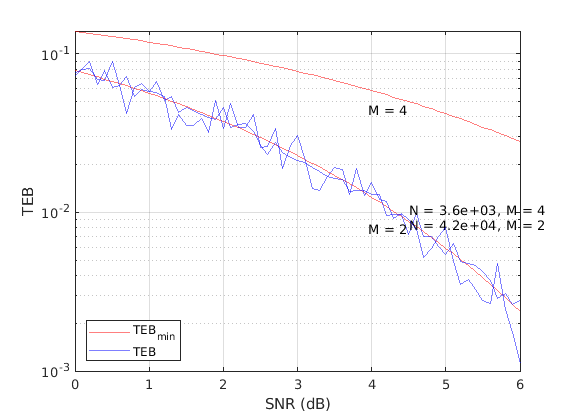
\includegraphics[width=0.8\textwidth]{graphics/1-5.png}
    \caption{TEB et TEB théorique en fonction du SNRB}
    \label{fig:teb_snrb_dvbs}
\end{figure}

On observe que le TEB par bit de la chaîne de transmission suit la courbe
théorique correspondant à une ordre de modulation $M = 2$ pour un mapping en
Amplitude Shift Keying (ASK). C'est en fait attendu, car le mapping QPSK permet
de répartir un plus grand nombre de symboles ($M = 4$) sur une constellation de
même taille. \medbreak

\clearpage
\section{Implantation de la chaîne passe-bas équivalente}

Nous conservons les mêmes paramètres que précédemment, excepté la fréquence
d'échantillonnage qui est ici $F_e = 6kHz$. Nous allons modéliser la même chaîne
de transmission, mais en utilisant un passe-bas équivalent. \medbreak

Le principe est d'ôter l'étape de transposition de fréquence, et de considérer
que le signal transmis est en bande de base. Pour maintenir un bruit
effectivement identique, nous devons utiliser un bruit complexe dans le canal de
transmission. \medbreak

Le signal émis est donc du même type que précédemment mais avec une DSP centrée
autour de $0Hz$:


\begin{figure}[H]
\begin{adjustbox}{center}
\subfloat{
    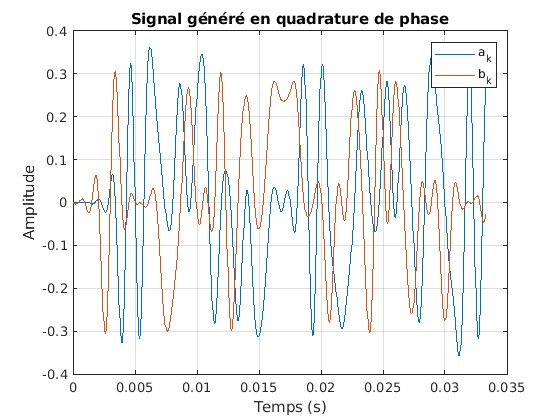
\includegraphics[width=0.6\textwidth]{graphics/2-1.jpg}
}
\hspace{-2em}
\subfloat{
    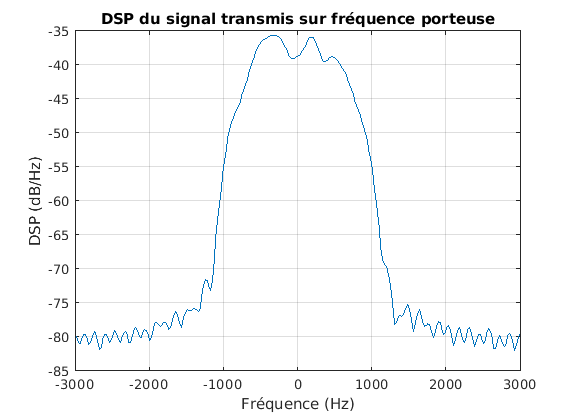
\includegraphics[width=0.6\textwidth]{graphics/2-2.png}
}
\end{adjustbox}
\end{figure}

Visualisons maintenant les constellations correspondant aux symboles en sortie
du mapping et en sortie de l'échantillonnage optimal (pour rappel, notre mapping
est en 4-PSK, donc il manque une rotation de $\frac{\pi}{4}$ pour obtenir les
symboles en QPSK).

\begin{figure}[H]
    \centering
    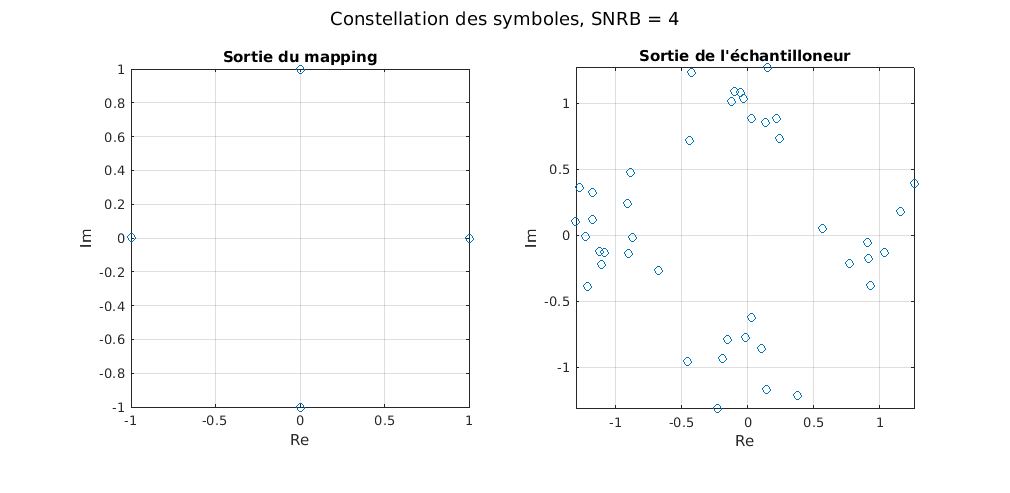
\includegraphics[trim=70 0 70 0, clip, width=0.8\textwidth]{graphics/2-4_4.png}
    \label{fig:constellation_dvbs}
\end{figure}

\vspace*{-1cm}
\begin{figure}[H]
\begin{adjustbox}{center}
\subfloat{
    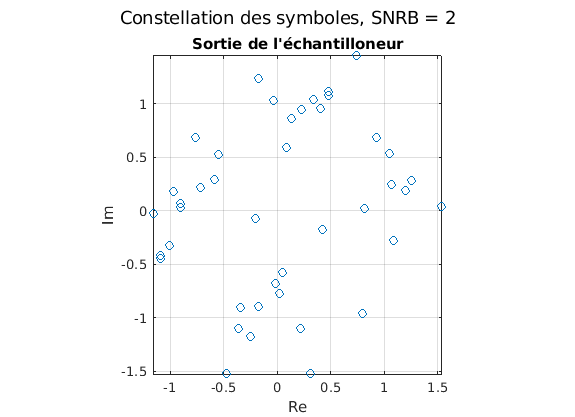
\includegraphics[trim=80 0 80 0, clip, width=0.4\textwidth]{graphics/2-4_2.png}
}
\subfloat{
    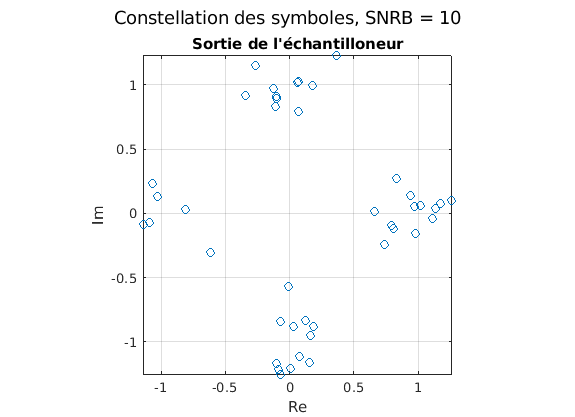
\includegraphics[trim=80 0 80 0, clip, width=0.4\textwidth]{graphics/2-4_10.png}
}
\end{adjustbox}
\end{figure}

Comme attendu, les symboles en sortie du mapping sont répartis sur une
constellation de 4 points sur le plan complexe, avec leurs arguments consécutifs
séparés de $\frac{\pi}{2}$. En sortie de l'échantillonnage optimal, les symboles
suivent une distribution gaussienne autour des points de la constellation du
mapping d'origine. La variance autour de chaque point est proportionnelle à la
puissance du bruit, et donc au $\operatorname{SNRB}$. Plus le $\operatorname{SNRB}$
est élevé, plus les symboles sont proches des points de la constellation, et
inversement. \medbreak

\clearpage
Le profil du TEB en fonction du $\operatorname{SNRB}$ est identique à celui
obtenu précédemment, ce qui est attendu car les deux chaînes de transmission
sont équivalentes. \medbreak

\begin{figure}[H]
    \centering
    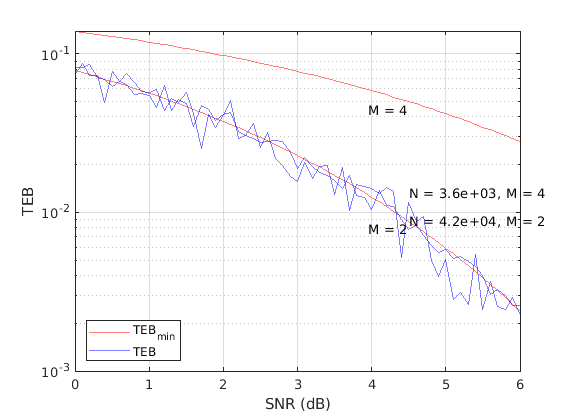
\includegraphics[width=0.8\textwidth]{graphics/2-5.png}
    \caption{TEB et TEB théorique en fonction du SNRB}
    \label{fig:teb_snrb_dvbs2}
\end{figure}

Ici, les chaînes de transmission sont équivalentes car on utilise un bruit blanc
gaussien uniforme sur toutes les fréquences. En réalité, le bruit dépend de la
bande de fréquence consdiérée, et transposer le signal en fréquence peut
permettre de réduire son impact sur le signal émis. \medbreak


\clearpage
\section{Comparaison du modulateur DVB-S avec un modulateur 4-ASK}

L'implémentation du modulateur 4-ASK revient à modifier uniquement le mapping
utilisé pour la modulation, qui s'effectue désormais en amplitude et non plus en
phase. Les symboles en sortie du mapping sont de la forme $d_k = a_k$ avec
$a_k \in \{-3, -1, 1, 3\}$. \medbreak

On obtient les constellations suivantes:

\begin{figure}[H]
    \centering
    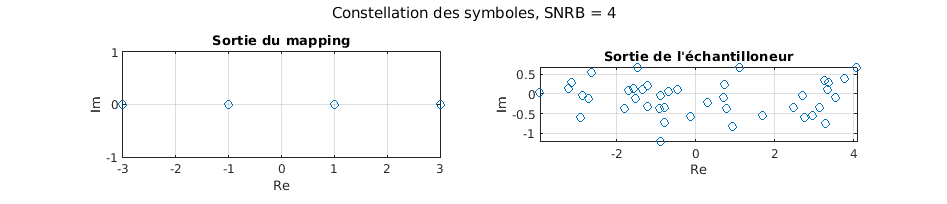
\includegraphics[trim=60 0 60 0, clip, width=\textwidth]{graphics/3-1_4.png}
    \label{fig:constellation_ask}
\end{figure}

\vspace*{-1cm}
\begin{figure}[H]
\begin{adjustbox}{center}
\subfloat{
    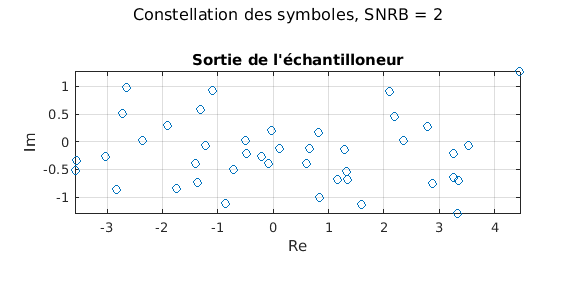
\includegraphics[trim=35 0 35 0, clip, width=0.5\textwidth]{graphics/3-1_2.png}
}
\hspace{1em}
\subfloat{
    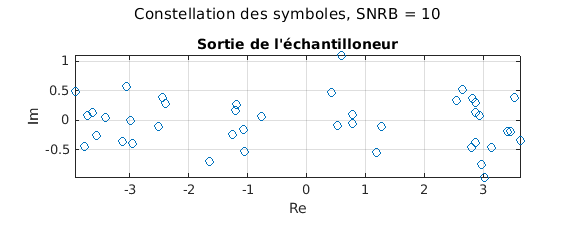
\includegraphics[trim=35 0 35 0, clip, width=0.5\textwidth]{graphics/3-1_10.png}
}
\end{adjustbox}
\end{figure}

Les symboles en sortie du mapping sont répartis sur une constellation de 4
points, tous sur la droite réelle, séparés de $2$ unités. En sortie de
l'échantillonnage, les symboles suivent toujours une distribution gaussienne
autour des points de la constellation du mapping. \medbreak

\clearpage
Évaluons le TEB en fonction du $\operatorname{SNRB}$:

\begin{figure}[H]
    \centering
    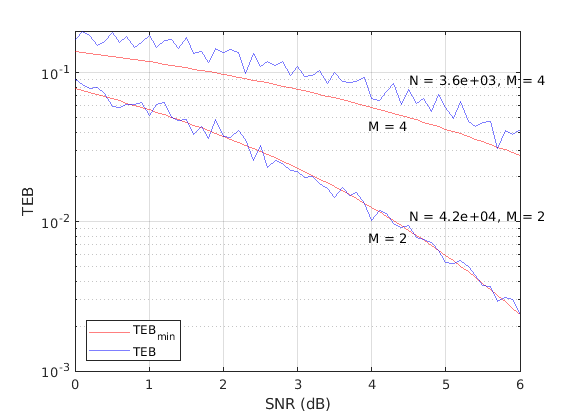
\includegraphics[width=0.8\textwidth]{graphics/3-2.png}
    \caption{TEB et TEB théorique en fonction du SNRB}
    \label{fig:teb_snrb_ask}
\end{figure}

Ici, le TEB pour un ordre de modulation $M$ suit bien la courbe théorique
correspondante. Le bruit est globalement plus important que pour le QPSK, car
les symboles sont plus éloignés les uns des autres avec un mapping en 4-ASK. En
effet, on utilise ainsi plus d'énergie pour transmettre un symbole, ce qui rend
le système plus sensible au bruit. On remarque donc que le QPSK présente une
meilleure efficacité en puissance que le 4-ASK. \medbreak

En termes d'efficacité spectrale, les deux modulateurs QPSK et 4-ASK sont
équivalents, car ils transmettent le même nombre de bits par symbole et utilisent
le même filtre de mise en forme. \medbreak

Il est clair que le QPSK est plus adapté à une transmission par satellite, car
il permet de transmettre plus d'information avec une puissance équivalente. \medbreak

\clearpage
\section{Comparaison du modulateur DVB-S avec un des modulateurs DVB-S2}

Le DVB-S2 est une évolution du DVB-S, qui remplace le mapping QPSK par un
mapping 8-PSK, et change la forme du filtre d'émission pour un filtre en racine
de cosinus surélevé de roll-off $\alpha = 0.2$. \medbreak

On obtient les constellations suivantes:

\begin{figure}[H]
    \centering
    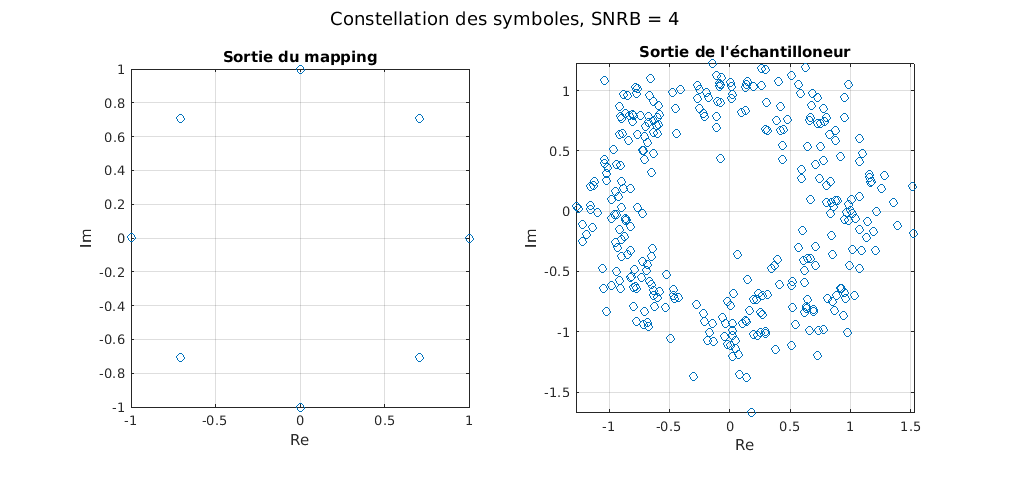
\includegraphics[trim=70 0 70 0, clip, width=0.8\textwidth]{graphics/4-1_4.png}
    \label{fig:constellation_dvbs2}
\end{figure}

\vspace*{-1cm}
\begin{figure}[H]
\begin{adjustbox}{center}
\subfloat{
    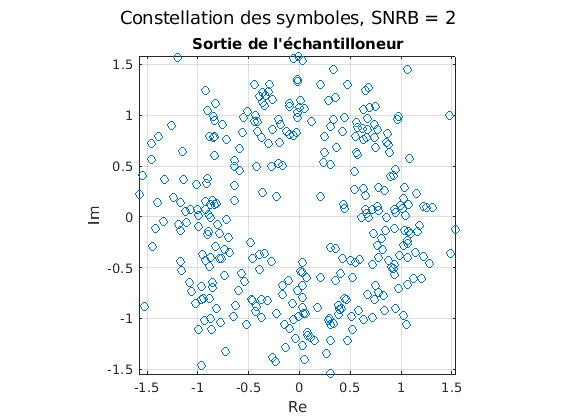
\includegraphics[trim=80 0 80 0, clip, width=0.4\textwidth]{graphics/4-1_2.png}
}
\subfloat{
    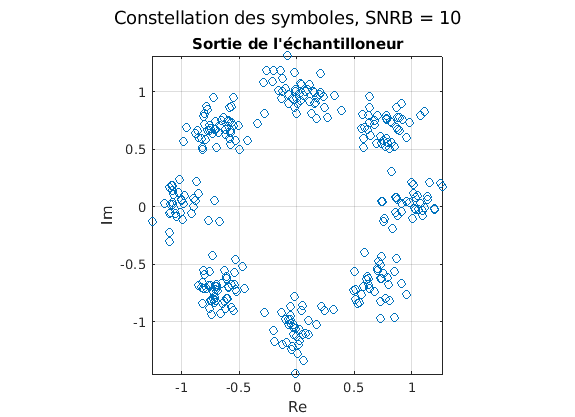
\includegraphics[trim=80 0 80 0, clip, width=0.4\textwidth]{graphics/4-1_10.png}
}
\end{adjustbox}
\end{figure}

La seule différence notable est que le nombre de symboles issu du mapping est
désormais de 8, répartis de manière uniforme sur un cercle de rayon 1, avec leurs
arguments consécutifs séparés de $\frac{\pi}{4}$, non plus de $\frac{\pi}{2}$. \medbreak

Évaluons le TEB en fonction du $\operatorname{SNRB}$:

\begin{figure}[H]
    \centering
    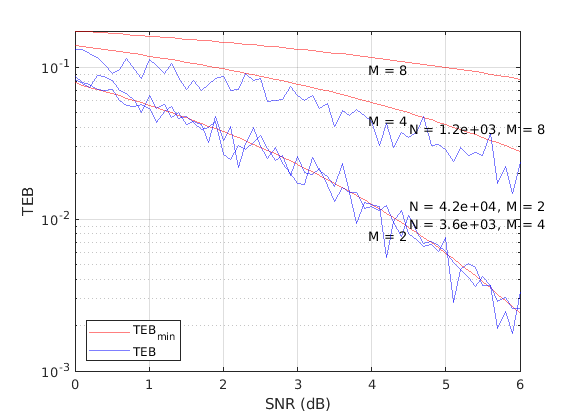
\includegraphics[width=0.8\textwidth]{graphics/4-2.png}
    \caption{TEB et TEB théorique en fonction du SNRB}
    \label{fig:teb_snrb_dvbs2}
\end{figure}

Par la même logique que pour le mapping QPSK, le TEB pour le DVB-S2, d'ordre de
modulation $M = 8$, suit la courbe théorique correspondante à un mapping en
4-ASK. On en conclut que le DVB-S2 est plus sensible au bruit que le DVB-S, et
présente une moins bonne efficacité en puissance. \medbreak

Cependant, comme l'ordre de modulation est plus élevé que pour le QPSK, le
DVB-S2 présente une meilleure efficacité spectrale que le DVB-S.

\begin{figure}[H]
    \centering
    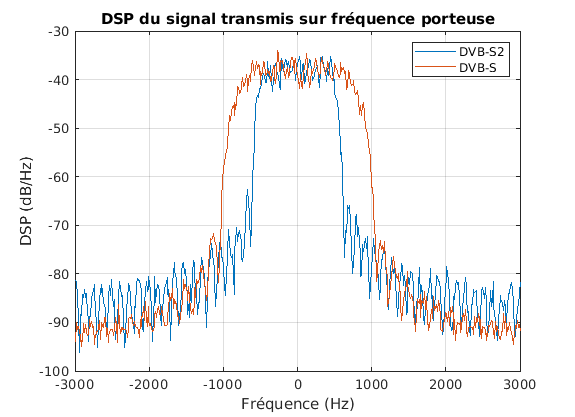
\includegraphics[width=0.8\textwidth]{graphics/4-3.png}
    \caption{Comparaison DSP entre DVB-S et DVB-S2}
    \label{fig:dsp_dvbs_dvbs2}
\end{figure}

En conclusion, décider d'utiliser des modulations plus complexes (avec un ordre
de modulation plus élevé) dépend des contraintes du système de transmission. Si
la puissance est limitée, il est préférable d'utiliser des modulations plus
simples comme le DVB-S. Si la puissance le permet, et qu'on souhaite transmettre
plus d'information dans une bande de fréquence donnée, ou réduire la bande
passante nécessaire, il est préférable d'utiliser des modulations plus complexes
comme le DVB-S2.

\end{document}
